\begin{figure}
    \centering
    \begin{subfigure}{.45\textwidth}
        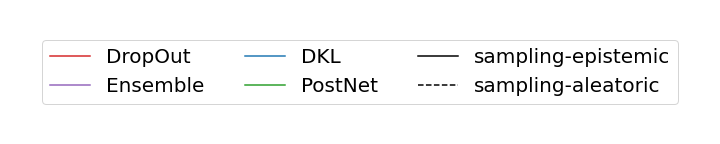
\includegraphics[width=\textwidth]{sections/011_icml2022/resources/sampling-legend.png}
    \end{subfigure}
    \vspace{-3mm}
    
    \begin{subfigure}{.245\textwidth}
        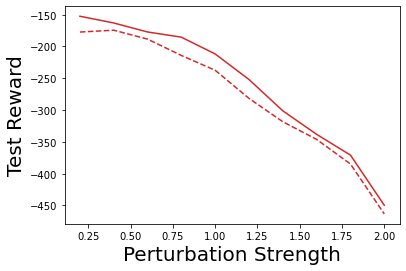
\includegraphics[width=\textwidth]{sections/011_icml2022/resources/action_shift-DropOut-AcrobotShift-v0-mean_reward_.png}
    \end{subfigure}
    \begin{subfigure}{.245\textwidth}
        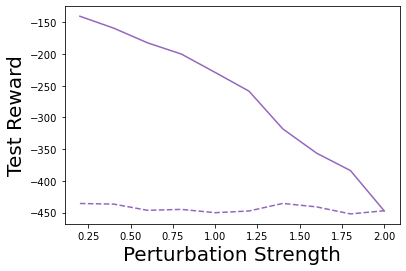
\includegraphics[width=\textwidth]{sections/011_icml2022/resources/action_shift-Ensemble-AcrobotShift-v0-mean_reward_.png}
    \end{subfigure}
    \begin{subfigure}{.245\textwidth}
        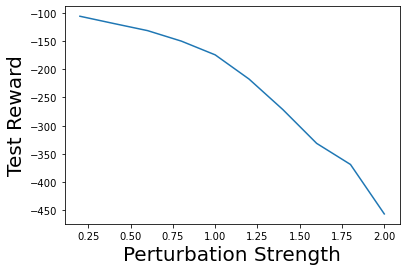
\includegraphics[width=\textwidth]{sections/011_icml2022/resources/action_shift-DKL-AcrobotShift-v0-mean_reward_.png}
    \end{subfigure}
    \begin{subfigure}{.245\textwidth}
        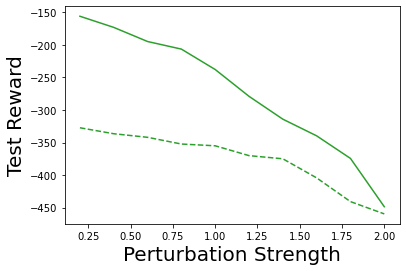
\includegraphics[width=\textwidth]{sections/011_icml2022/resources/action_shift-PostNet-AcrobotShift-v0-mean_reward_.png}
    \end{subfigure}
    
    \begin{subfigure}{.245\textwidth}
        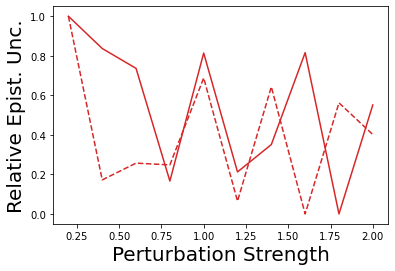
\includegraphics[width=\textwidth]{sections/011_icml2022/resources/action_shift-DropOut-AcrobotShift-v0-mean_epistemic_uncertainty_.png}
    \end{subfigure}
    \begin{subfigure}{.245\textwidth}
        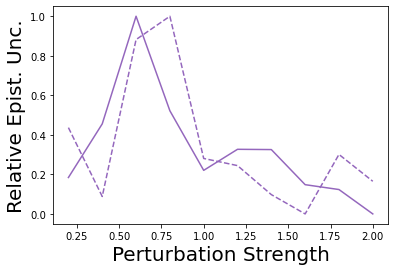
\includegraphics[width=\textwidth]{sections/011_icml2022/resources/action_shift-Ensemble-AcrobotShift-v0-mean_epistemic_uncertainty_.png}
    \end{subfigure}
    \begin{subfigure}{.245\textwidth}
        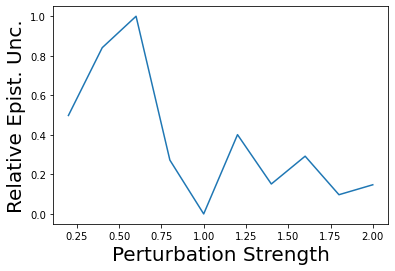
\includegraphics[width=\textwidth]{sections/011_icml2022/resources/action_shift-DKL-AcrobotShift-v0-mean_epistemic_uncertainty_.png}
    \end{subfigure}
    \begin{subfigure}{.245\textwidth}
        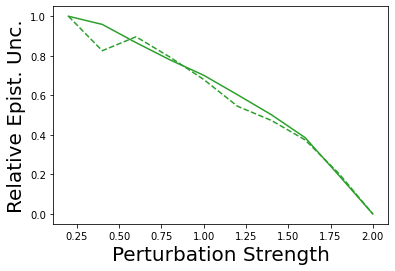
\includegraphics[width=\textwidth]{sections/011_icml2022/resources/action_shift-PostNet-AcrobotShift-v0-mean_epistemic_uncertainty_.png}
    \end{subfigure}
    \caption{Comparison of the testing performance and the epistemic uncertainty predictions on Acrobot with perturbed actions. The four uncertainty methods use the epsilon-greedy strategy at training time and the sampling-aleatoric or sampling-epistemic strategy at testing time. Ideally, an uncertainty-aware model should maintain high reward while assigning higher epistemic uncertainty on more severe perturbations.}
    \label{fig:strategy-action-shift-testing-performance-acrobot}
\end{figure}